\section{Molmassen wichtiger Atome}

\begin{tabular}{c | c | c }
\textbf{Symbol} & \textbf{Molekül} & \textbf{Molmasse} \\
\hline
\rule{0pt}{10pt} H & Wasserstoff & $1.008 \, \mathrm{\frac{g}{mol}}$ \\
\rule{0pt}{10pt} C & Kohlenstoff & $12.011 \, \mathrm{\frac{g}{mol}}$ \\
\rule{0pt}{10pt} N & Stickstoff & $14.007 \, \mathrm{\frac{g}{mol}}$ \\
\rule{0pt}{10pt} O & Sauerstoff & $15.999 \, \mathrm{\frac{g}{mol}}$ \\
\rule{0pt}{10pt} Al & Aluminium & $26.982 \, \mathrm{\frac{g}{mol}}$ \\
\rule{0pt}{10pt} Si & Silicium & $28.982 \, \mathrm{\frac{g}{mol}}$ \\
\end{tabular}

\vfill\null
\columnbreak



\section{Ansätze zu Aufgaben}

\subsection{Barometer}
\begin{minipage}{0.4\linewidth}
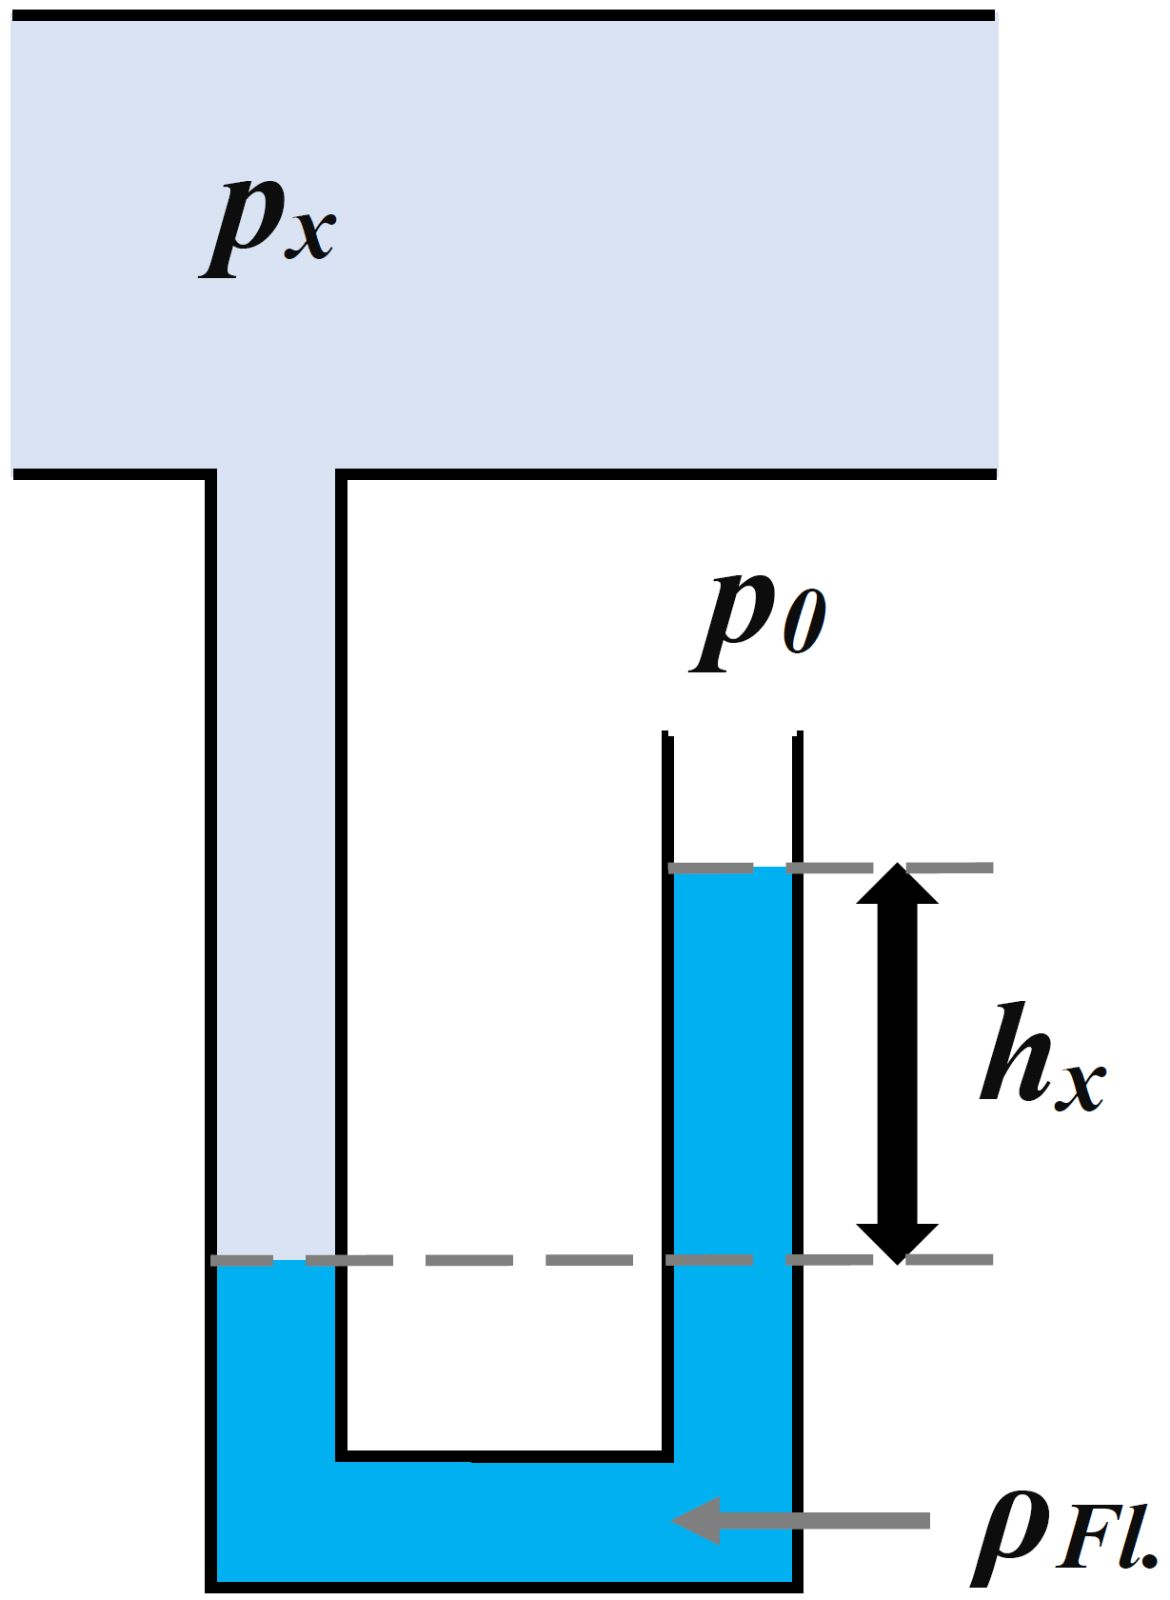
\includegraphics[width=\linewidth]{Bilder/manometer} \\
\end{minipage}
\hfill
\begin{minipage}{0.5\linewidth}
$\boxed{ p_1 = p_0 + \underbrace{ \rho_{Fl} \cdot g \cdot h}_{\substack{p_s}} }$
 
 
\begin{tabular}{ll}
\\
$p_1$ & gemessener Druck \\
$p_0$ & Luftdruck \\
$p_s$ & Schweredruck \\
\\
\end{tabular}

$\Rightarrow$ Bernoulli \\
$\Rightarrow$ Kontinuität \\
\\
\\
\\
\\
\\
\end{minipage}




\subsection{Pitotrohr}
Prandtl'sches Staurohr; Staudruckmesser \\
Zur Messung von Strümungsgeschwindigkeiten \\
\\
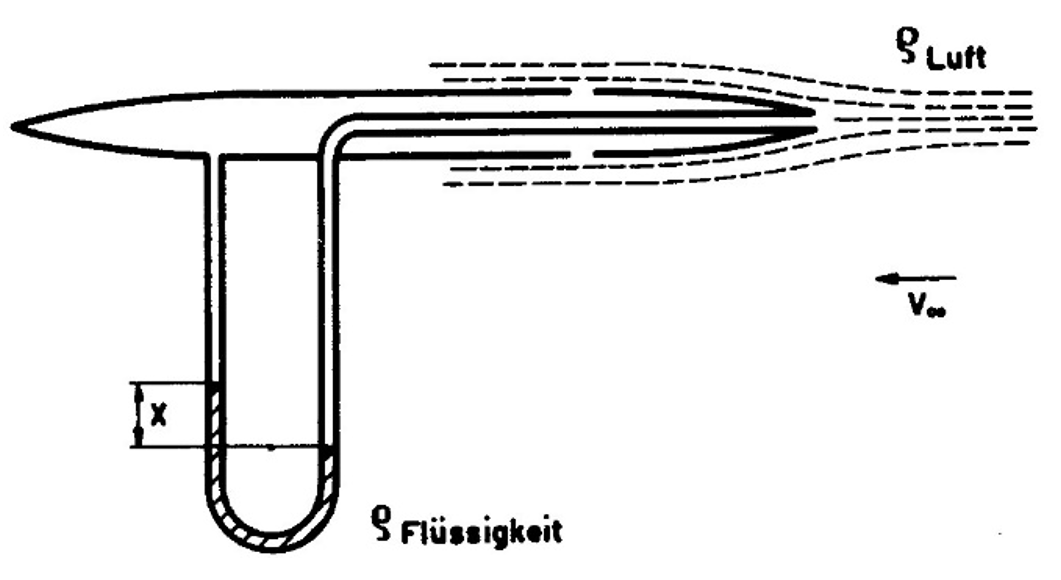
\includegraphics[width=0.73\linewidth]{Bilder/pitotrohr} \\

$$ \mathrm{Bernoulli \; horizontal:} \quad \boxed{  \underbrace{p_1}_{\substack{p_L}} + \frac{1}{2} \, \rho_1 \cdot \underbrace{v_1^2}_{\substack{0}} =  \underbrace{p_2}_{\substack{p_L - \Delta p}} + \frac{1}{2} \, \underbrace{\rho_2}_{\substack{\rho_L}} \cdot v_2^2} $$

$$ 0 = - \Delta p + \frac{1}{2} \, \rho_L \cdot v_2^2 \qquad \Rightarrow \Delta p =\frac{1}{2} \, \rho_L \cdot v_2^2 $$

$$ \mathrm{Gleichsetzen: } \quad \Delta p = \rho_{Fl} \cdot g \cdot h$$


\subsection{Pumpe}
$$ \boxed{ W = P \cdot t = F \cdot \Delta s = p \cdot A \cdot \Delta s = p \cdot \Delta V }  $$

$$ \boxed{ P =  \frac{W}{t} = \frac{p \cdot V}{t} = p  \cdot  \dot{V} } $$

$$ \boxed{ F = p \cdot A } $$

\vfill\null
\columnbreak


\subsection{Bewegungen}

$$ \boxed{ P = F \cdot v } $$

$$ \boxed{ E_{kin} = \frac{1}{2} \, m \cdot v^2 } $$


\subsection{U-Rohr}

\begin{minipage}{0.4\linewidth}
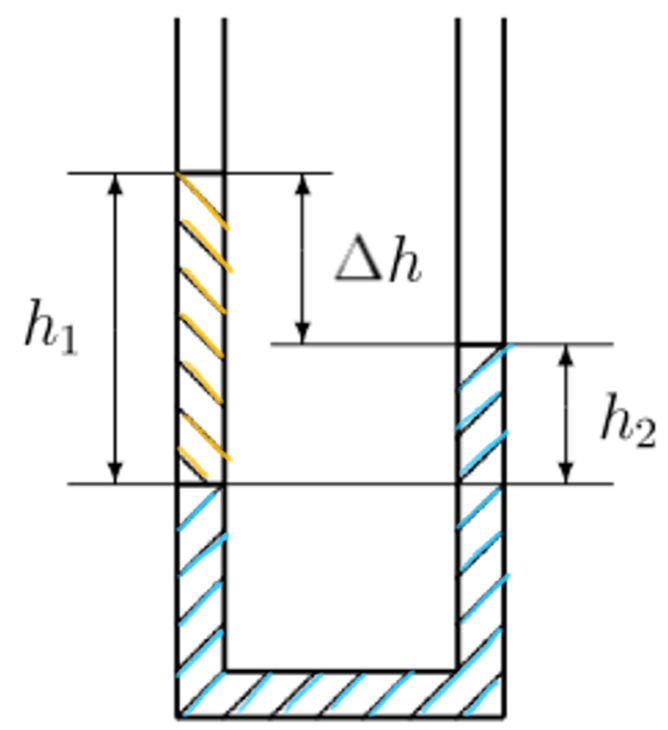
\includegraphics[width=\linewidth]{Bilder/u-rohr} \\
\end{minipage}
\hfill
\begin{minipage}{0.55\linewidth}
Ansatz: Druckgleichgewicht 

$$ p_1 = p_2 $$

$$ \rho_1 \cdot g \cdot h_1 = \rho_2 \cdot g \cdot h_2  $$
\end{minipage}


\subsection{Wasser mit Dampf erhitzen}

Ein Tasse mit $m_W = 200 \, \mathrm{g}$ Wasser  mit einer Temperatur von $T_K = 20 \, \text{°C}$ wird an
der Wasserdampfdüse einer Kaffeemaschine mittels Wasserdampf erhitzt. Der aus der
Kaffeemaschine ausströmende Wasserdampf ist $T_H = 96 \, \text{°C}$ heiss. Am Schluss haben sie 10 \%
mehr Wasser in der Tasse. (entspricht $m_D$)\\
Wie warm ist das Wasser nun? \\
\\
Ansatz: 1. Hauptsatz \quad $Q_{zu} = Q_{ab}$ \\
\\
$$ m_W \cdot c_W \, (T_M - T_K) = q_s \cdot m_D + m_D \cdot c_W \, (T_H - T_M) $$



\subsection{Eis in Wasser schmelzen}

In einem Gefäss beifinden sich $m_W = 1 \, \mathrm{kg}$ Wasser. Dazu wird ein Eiswürfel von $m_E = 20 \, \mathrm{g}$ gegeben. Das Eis hat eine Temperatur von $T_E = -5 \, \text{°C}$ und das Wasser hat eine Temperatur $T_W$. Die Temperatur $T_0$ steht für $0 \, \text{°C}$ bzw. 275.15 K \\
Gesucht ist die Mischtemperatur $T_M$ 

$$ \Delta Q_{ab} = \Delta Q_{zu}$$
$$ m_W \cdot c_W \cdot (T_W - T_M) = m_E \cdot c_E \cdot (T_E - T_0) + q_f \cdot m_E + c_W \cdot (T_M - T_0) $$
